\chapter{Adventuring}\label{Adventuring}

This chapter describes how to play Rise outside of combat situations.
It also provides general advice about how Rise games are typically run.
For information about how characters are defined, including their statistics, see \pcref{Characters}.
To run combat scenarios, see \pcref{Combat}.

\section{Defining the Undefined}
    This book does not attempt to include specific rules for every aspect of a realistic world.
    Unless defined otherwise - or if it's not worth the effort to look up Rise's exact rules in the flow of a game - you should assume that the universe works more or less like the real world does, and as long as everyone agrees that something is reasonable, it's not worth worrying about in more detail.

    For example, Rise does not have specific rules for how long it takes to eat a meal, the arc that a thrown ball takes through the air, or how much extra weight a well-made chandelier can hold without breaking.
    It's possible to imagine situations where each of those might be important to a game, however, so you'll have to guess what would be reasonable as obscure situations arise.
    The Game Master has the final word when defining ambiguities like this.

    \subsection{Resolving Ambiguity}\label{Resolving Ambiguity}
        When the rules are ambiguous about how they apply to you and no other creature, you decide how to resolve that ambiguity.
        For example, if an ability causes you to remove one of your \glossterm{vital wounds}, and you have more than one vital wound, you choose which vital wound is removed.
        When the rules are ambiguous in any other situation, the GM decides how to resolve that ambiguity.
        This includes situations where multiple creatures are relevant and situations where no particular creature is relevant.

\section{Making Checks}\label{Checks}\label{Making Checks}
    Checks are required to perform actions that have a chance of failure where the difficulty is not measured by the defense of another creature or object.
    For example, climbing a wall or remembering an obscure piece of trivia may require a check.

    To make a check, roll 1d10 and add your modifier with the check.
    You compare that result to a \glossterm{difficulty value} that represents the difficulty of the task.
    The more difficult the task, the higher the \glossterm{difficulty value} will be.
    If your result is equal to or higher than the \glossterm{difficulty value}, the check succeeds.
    This usually means you accomplish a task successfully.
    Otherwise, the check fails.
    This usually means that nothing happens, though sometimes there are specific consequences for failure.

    \subsection{Critical Success}
        If your check result is at least 10 higher than the \glossterm{difficulty value}, your check is a \glossterm{critical success}.
        Some checks have a special effect on a critical success.
        For example, a critical success while climbing means you move twice as quickly (see \pcref{Climb}).

    \subsection{Standard Difficulty Values}\label{Standard Difficulty Values}
        Most checks are made against a fixed \glossterm{difficulty value} that represents how hard the task is.
        Detailed rules for determining difficulty values in specific circumstances can be found in the Expanded Skills chapter from the Tome of Guidance.
        However, most of the time, it's not worth the effort to consult charts and tables to figure out how hard a task is.
        Instead, you can estimate it based on the guidelines below.

        \begin{itemize}
            \item DV 0 - Easy: Only an exceptionally incompetent or impaired person could possibly fail a DV 0 check. For example, this includes walking on rough ground without tripping (Balance) or noticing that a yelling, red-faced person is angry (Social Insight).
            \item DV 5 - Average: A typical human with no relevant skills should still succeed at a DV 5 check without much issue. However, it would be possible to fail in a stressful situation where time is limited if the person had no relevant training. For example, this includes climbing a ladder (Climb) or hearing the topic of a nearby conversation in a crowded bar (Awareness).
            \item DV 10 - Hard: A typical human with no relevant skills might succeed at a DV 10 check, but only if they were very lucky or had a lot of time on their hands. An experienced practicioner might fail infrequently in stressful circumstances, but a world-class expert would never fail. For example, this includes swimming in fast-moving water (Swim) or providing first aid to mitigate a barely lethal wound (Medicine).
            \item DV 15 - Very Hard: Only an experienced practicioner could succeed at a DV 15 check, and they would still need to get lucky if they were in a rush. Even a world-class expert at the peak of real-world human potential could fail, but only rarely. For example, this includes picking a well-made lock (Devices) or holding your breath for eight minutes while staying still (Endurance).
            \item DV 20 - Almost Impossible: A world-class expert like an Olympic medalist could succeed at a DV 20 check if they were lucky or patient. Succeeding consistently at tasks of this difficulty requires superhuman capabilities. For example, this includes climbing a weathered natural rock wall without equipment (Climb) or squeezing through a space with a diameter of only half a foot (Flexibility).
            \item DV 25\add - Impossible: No real-world human can succeed at a DV 25 check. This sort of feat is only possible for high-level Rise characters who have explicitly surpassed ordinary limitations. For example, this includes running at full speed along a slack rope (Balance) or climbing a sheer glass pane (Climb).
        \end{itemize}

    \subsection{Trying Again}
        You can think of checks as being broadly divided into two categories: checks that give you information, and checks that cause a change in the world around you.
        In general, you can retry checks that change your environment indefinitely until you succeed.
        The only major limiting factor to those checks is that failure sometimes also changes your environment in ways that may punish your failure or make it impossible to retry the check.
        For example, if you are trying to climb a cliff, you can keep trying until you succeed, but you may take \glossterm{falling damage} from falling off while halfway up the cliff.

        You generally cannot retry checks that give you information unless the situation changes in a way that is relevant to your check.
        This often takes the form of giving you new information.
        For example, if you've already examined a creature to determine whether they are disguised, you can't keep just keep staring that creature to make sure.
        However, if you splash the creature with water which washes away some makeup, you can try again now that you have more information.

        % TODO: it would be nice if this wasn't necessary
        In addition, checks that require a free action to make can never be made more than once for the same purpose within a round.

    \subsection{Opposed Checks}
        An opposed check involves multiple creatures competing to get the highest result.
        In case of a tie, all tied creatures roll again to break the tie.
        Usually, the creature with the highest result succeeds, while all other creatures either fail completely or simply succeed less effectively depending on the situation.

        Some opposed checks involve multiple creatures using the same skill to see who does the best job.
        For example, a climbing race up a wall might involve each participant rolling a Climb check, or you might make a Strength check to hold a door closed while another creature tries to shove it open.
        Alternately, it can involve creatures rolling opposite skills.
        For example, if you are trying to hide, you roll a Stealth check opposed by the Awareness check of any creatures who could notice you.

        Not all opposed checks require all participants to roll at the same time.
        For example, a creature who creates a disguise rolls the Disguise check at the time that the disguise is created.
        A creature who tries to notice the disguise would roll their Awareness check at the time they see the disguised creature.

    \subsection{Hidden Checks}
        The GM can always make checks on your character's behalf without telling you.
        Generally, this is used for observation-based skills.
        For example, it's very suspicious if the GM tells you to make an Awareness check and then tells you that you don't see anything interesting.
        One of the ways a GM can avoid that is by simply rolling a check on behalf of your character and only telling you the result if you succeed.

    \subsection{Helping On Checks}
        You can help an \glossterm{ally} make a check.
        To help an ally, you make a check of the same type against a \glossterm{difficulty value} that is 5 lower than the regular difficulty value.
        This has the same requirements, including time and physical contact, as the check would have if you made it yourself.
        For example, to help an ally climb a cliff, you must be able to touch your ally to guide them up.
        Success means that the ally gains a \plus2 bonus to the check.

        Multiple creatures can try to help the same person.
        At the GM's discretion, there may be a practical limit to how many people can assist with the same task.
        The bonus from multiple creatures helping does not stack.
        It just makes it more likely that the helping attempt will succeed.

    \subsection{Checks for Timed Tasks}
        For every 5 points by which you beat the \glossterm{difficulty value} to accomplish a timed task, the time required is usually halved.
        This only applies for tasks that have a base time requirement of at least one minute, if the GM agrees that it is relevant, and if there are no other specific ways in which your result is improved with higher check results.

\section{Resting}\label{Resting}
    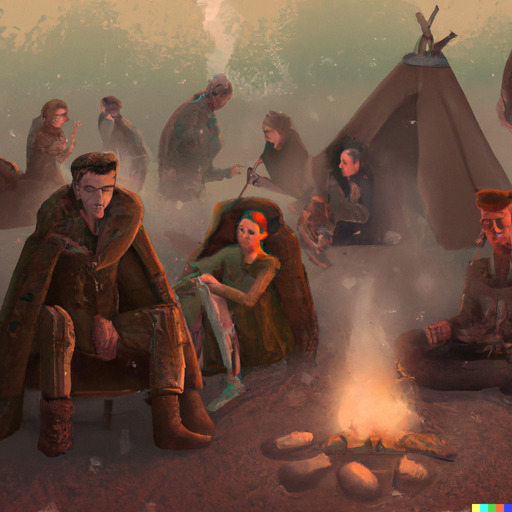
\includegraphics[width=\columnwidth]{core mechanics/resting}

    When you have a moment to relax, you can rest to regain some of your expended resources.
    There are two main types of rests: a \glossterm{short rest} and a \glossterm{long rest}.
    The benefits of taking a short rest or long rest happen automatically after you spend enough time avoiding strenuous activity.
    You do not have to declare that you are using the ``short rest'' or ``long rest'' ability.
    Resting at night is often combined with sleeping, but you can rest at any time without sleeping.

    % TODO: clarify interrupted rests

    \subsection{Short Rest}\label{Short Rest}
        Resting for ten minutes is considered a \glossterm{short rest}.
        When you finish a short rest, you gain the following benefits.
        \begin{itemize}
            \item Your \glossterm{hit points} become equal to your maximum hit points.
            \item Your current \glossterm{damage resistance} becomes equal to your maximum damage resistance.
            \item You regain any \glossterm{attunement points} you released from \glossterm{deep attunement} effects (see \pcref{Deep Attunement}).
            \item You remove all \glossterm{conditions} affecting you.
            \item Some other abilities have specific effects that last until you finish a short rest.
        \end{itemize}

    \subsection{Long Rest}\label{Long Rest}
        Resting for eight hours is considered a \glossterm{long rest}.
        When you finish a long rest, you gain the following benefits.
        \begin{itemize}
            \item You remove one of your vital wounds (see \pcref{Removing Vital Wounds}).
                The Medicine skill can increase this healing (see \pcref{Accelerate Recovery}).
            \item Your \glossterm{fatigue level} becomes 0.
            \item Some other abilities have specific effects that last until you finish a long rest.
        \end{itemize}

        You can take multiple long rests consecutively to recover from extensive vital wounds.

    \subsection{Sleep and Fatigue}\label{Sleep and Fatigue}
        A typical creature needs a minimum of 6 hours of sleep for every 18 hours spent awake, and a minimum of 50 hours of sleep every week.
        You can stay awake beyond those limits with the Endurance skill (see \pcref{Stay Awake}).

\section{Communication and Languages}\label{Languages}\label{Communication and Languages}

    \parhead{Literacy}
    All characters with an Intelligence of \minus2 or higher are presumed to be literate, allowing them to read and write any language they speak. Each language has an alphabet, though sometimes several spoken languages share a single alphabet.

    \parhead{Language Rarity}\label{Language Rarity}
    Some languages are widely spoken in the world, while others are only encountered in unusual circumstances.
    Common languages are summarized on \trefnp{Common Languages}, below.
    Rare languages are summarized on \trefnp{Rare Languages}, below.
    Rare languages are more difficult to learn, and are usually only spoken by unusual creatures.

    \parhead{Learning Languages}\label{Learning Languages}
    Learning a language is a time-consuming process, and most characters only know a few languages based on their species.
    You can learn two common languages or one rare language in place of training a skill (see \pcref{Skills}).
    In addition, you can talk to your GM about knowing an additional language based on your character's personal background.

    \begin{dtable}
        \lcaption{Common Languages}
        \begin{dtabularx}{\columnwidth}{l >{\lcol}X l}
            \tb{Language} & \tb{Typical Speakers} & \tb{Alphabet} \tableheaderrule
            Common        & Civilized creatures   & Common   \\
            Draconic      & Dragons, kobolds      & Draconic \\
            Dwarven       & Dwarves               & Dwarven  \\
            Elven         & Elves                 & Elven    \\
            Giantish      & Ogres, giants         & Dwarven  \\
            Gnoll         & Gnolls                & Common   \\
            Gnome         & Gnomes                & Dwarven  \\
            Goblin        & Goblins, hobgoblins   & Dwarven  \\
            Halfling      & Halflings             & Common   \\
            Orcish        & Orcs                  & Dwarven  \\
        \end{dtabularx}
    \end{dtable}

    \begin{dtable}
        \lcaption{Rare Languages}
        \begin{dtabularx}{\columnwidth}{l >{\lcol}X l}
            \tb{Language}  & \tb{Typical Speakers}  & \tb{Alphabet} \tableheaderrule
            Abyssal     & Evil planeforged      & Abyssal  \\
            Aquan       & Water-based creatures & Elemental \\
            Auran       & Air-based creatures   & Elemental \\
            Celestial   & Good planeforged      & Celestial \\
            Ignan       & Fire-based creatures  & Elemental \\
            Sylvan      & Dryads, faeries       & Elven     \\
            Terran      & Earth-based creatures & Elemental \\
            Undercommon & Drow                  & Elven
        \end{dtabularx}
    \end{dtable}

\section{Ability Mechanics}\label{Ability Mechanics}

    \subsection{Magical and Mundane Abilities}\label{Magical and Mundane Abilities}

        There are two types of abilities: magical abilities and mundane abilities.

        \parhead{Magical Abilities}\label{Magical Abilities} A \magical ability is an ability fundamentally composed of or fuelled by magic.
        Magical abilities often have effects that would be impossible without magical intervention.
        Examples include \glossterm{spells}, a dragon's ability to fly, and a paladin's ability to smite foes.
        Abilities that are magical in nature are indicated with a \sparkle in their name.
        Abilities that are not magical are \glossterm{mundane}.

        \parhead{Mundane Abilities}\label{Mundane Abilities} A \glossterm{mundane} ability has some form of natural explanation and does not fundamentally originate from a magical source.
        Examples include weapon attacks, a dragon's frightful presence, and a barbarian's rage.
        Unless otherwise indicated, all abilities are mundane in nature.
        Abilities that are not mundane are \magical.

    \subsection{Targets}\label{Targets}
        Almost all abilities affect targets.
        A target of an ability is a creature directly affected by the ability in some way.
        Many abilities affect targets within a specific \glossterm{range}.

        \subsubsection{Targeted Abilities}\label{Targeted Abilities}
            Some abilities allow you to choose specific targets.
            There can be restrictions on the targets of the ability, such as ``a creature or object'' or ``an \glossterm{ally}''.
            These abilities are called \glossterm{targeted} abilities.

        \subsubsection{Area Abilities}
            Some abilities affect all valid targets within a given area.
            There can be restrictions on the targets of the ability, such as ``all creatures'' or ``all \glossterm{enemies}''.
            However, you cannot individually choose to include or exclude specific targets.
            These abilities are not \glossterm{targeted} abilities.

        \subsubsection{Invalid Targets}
            % clarify timing
            You can always attempt to use an ability on an invalid target.
            If the target is still invalid when the ability resolves, the ability automatically fails and has no effect on the target.

        \subsubsection{Primary and Secondary Targets}\label{Primary and Secondary Targets}
            Some abilities that affect multiple targets distinguish between their primary and secondary targets.
            For example, the \spell{chain lightning} spell affects secondary targets within a small radius around a primary target.
            If an ability does not mention secondary targets, all of its targets are primary targets.

            Unless otherwise specified, abilities have the same effect on their primary and secondary targets.
            However, \glossterm{line of effect} for secondary targets is always measured from the primary target, rather than from the ability's source.
            \glossterm{Line of sight} is still measured from the ability's source.
            This can allow you to hit secondary targets behind walls if you can still see them or otherwise target them, and if there is no obstacle separating from the primary target.

    \subsection{Touch}\label{Touch}
        Some abilities specify that you must touch a target.
        You can only touch creatures that are adjacent to you.
        Touching a creature that is not an \glossterm{ally} requires an attack against the target's Reflex defense, which is usually mentioned as part of the ability's description.
        Some creatures cannot be touched, such as \glossterm{incorporeal} creatures.

    \subsection{Area}\label{Area}

        Some abilities affect targets within an area.
        All areas have a \glossterm{point of origin}, an area shape, a measurement of their size in feet, and an area type (see \pcref{Point of Origin}).

        \subsubsection{Area Shapes}\label{Area Shapes}

            \parhead{Cone} A cone extends from the point of origin in a quarter-hemisphere, up to the given length.
            A square is affected by a cone if it is within the cone's 90 degree arc and all of the square's points of intersection are no more than the cone's length away from the cone's point of origin.

            \parhead{Cylinder} A cylinder extends out from the point of origin in a circle, up to the given radius.
            Cylinders also have a specific height.
            Unless otherwise specified, a cylinder's height is the same as its radius.

            \parhead{Line} A line extends from the point of origin in a straight line, up to the given length.
            Lines also have a specific width and height.
            Unless otherwise specified, a line-shaped ability affects an area 5 feet wide and 5 feet high.
            The affected squares are chosen such that they stay close to the chosen line as possible.
            All squares affected by a line must be contiguous, so every square is adjacent to another affected square, disregarding diagonals.

            If a line-shaped effect has its area increased, only the length of the line increases unless otherwise noted.

            \parhead{Sphere} A sphere extends from the point of origin in all directions.
            Any ability which only specifies a radius for its area is sphere-shaped.

            \parhead{Wall} A wall is like a line, except that its width is not defined in squares.
            Narratively, all walls have a nonzero width.
            Mechanically, walls are considered to have no width and simply occupy the boundary between squares.
            Like lines, some walls are shapeable.

            All walls share the following common properties unless their description says otherwise.
            A wall's height is equal to half its length for straight walls, or half its radius for circular walls, to a minimum of 10 feet high.
            The entire wall is considered to be a single object, and is attacked and destroyed as a single unit.
            All of a wall's defenses are 0, but like other objects, they are immune to \glossterm{critical hits}.
            Most abilities that create walls indicate how many hit points the wall has.
            If an ability does not specify a wall's hit points, it does not have hit points and cannot be destroyed with damage.

            If you create a wall within a space too small to hold it, it fills as much of the space as possible, starting from the middle of the chosen space.
            This can allow you to completely block off small tunnels.

            Walls can normally be created within or adjacent to occupied squares, but not within solid objects.
            If a wall has hit points, it cannot be created inside the space of a single creature, but it can be created between two adjacent creatures.

            % \parhead{Specific Shapes} Some abilities specify a series of volumes that make up the area of the ability.
            % Most commonly, the volumes are cubes.
            % You may arrange the volumes as you want, with the restriction that each volume in the ability's area must be adjacent to one other volume in the ability's area.

        \subsubsection{Area Size}

            The area affected by many abilities falls into one of six sizes.
            Each size defines the extent to which the ability extends out from its origin, whether as a radius or as a length.
            Many abilities have specific sizes, as given in the ability description.

            \parhead{Tiny} Tiny areas extend 5 feet from their point of origin.
            \parhead{Small} Small areas extend 15 feet from their point of origin.
            \parhead{Medium} Medium areas extend 30 feet from their point of origin.
            \parhead{Large} Large areas extend 60 feet from their point of origin.
            \parhead{Huge} Huge areas extend 120 feet from their point of origin.
            \parhead{Gargantuan} Gargantuan areas extend 240 feet from their point of origin.

        \subsubsection{Area Types}\label{Area Types}

            \parhead{Burst} A burst ability has an immediate effect on all valid targets within an area.
            If an ability does not explicitly specify its area type, it is normally a burst effect.
            However, abilities that create wall-shaped areas are always zones.

            \parhead{Emanation} An emanation ability has effects within an area for the duration of the ability.
            It emanates from a specific creature or object, rather than a location.
            If that creature or object moves, the emanation moves with it.

            \parhead{Zone} A zone ability has effects within an area for the duration of the ability.
            Unless otherwise noted, it does not move after being created.

            When casting an area ability, you select the point where the ability originates.
            The point of origin of an ability is always a grid intersection.
            When determining whether a given creature is within the area of an ability, count out the distance from the point of origin in squares just as you do when moving a character or when determining the range for a ranged attack.
            The only difference is that instead of counting from the center of one square to the center of the next, you count from intersection to intersection.

            % This seems like an unnecessary complication, and is easily forgotten.
            % But it does solve some potentially unintuitive scenarios, like upgraded versions of spells not always being strictly better.
            % You can freely decrease a ability's area, provided that you decrease it uniformly across all of the ability's dimensions.
            % For example, you can cast a \spell{fireball} spell that affects a 5 foot radius if you choose to do so, but you can't cast a \spell{fireball} with any shape other than a sphere.

            You can count diagonally across a square, but remember that every second diagonal counts as 2 squares of distance.
            If the far edge of a square is within the ability's area, anything within that square is within the ability's area.
            If the ability's area only touches the near edge of a square, however, anything within that square is unaffected by the ability.

    \subsection{Ability Durations}\label{Ability Durations}

        An ability's duration determines how long its effect lasts.
        Abilities can have one of several different kinds of durations.

        % TODO: Is this necessary?
        % Should this clarify interactions with bursts/zones/emanations?
        If an ability targets creatures or objects directly, the effects travel with the subjects for the ability's duration, even if the subjects go outside the ability's initial range.
        If an ability creates or summons objects or creatures, they last for the duration of the ability, and are capable of moving outside the ability's initial range.
        Such effects can sometimes be destroyed prior to when their duration ends.

        \subsubsection{Attuned Abilities}
            Many abilities last as long as a creature \glossterm{attunes} to them.
            For details, see \pcref{Attunement}.

        \subsubsection{Conditions}\label{Conditions}
            Many abilities impose \glossterm{conditions} on their targets.
            A condition lasts until it is removed.
            You can remove conditions by taking a \glossterm{short rest} or using the \textit{recover} ability (see \pcref{Recover}).
            There are several other abilities that can also remove conditions.

        % TODO: clean up wording
        \subsubsection{Sustained Abilities}\label{Sustained Abilities}
            Sustained abilities have the \abilitytag{Sustain} tag.
            They last as long as you take an action to sustain them each round.
            The type of action required is always specified in the ability's tag, such as ``Sustain (standard)'' for a standard action, or in the ability's description.

            At the start of each \glossterm{action phase}, the ability is dismissed unless you take the appropriate action to sustain the ability.
            This happens before your normal turn, so you and your allies can't gain the benefits of a sustained ability without you sustaining it.

            Some sustained abilities include ``attuneable'' in the tag before the action type.
            When you use or sustain that ability, you can choose to \glossterm{attune} to it.
            If you do, it gains the \abilitytag{Attune} tag and loses the \abilitytag{Sustain} tag, so it stays active as long as you stay attuned to it.

            Taking an action to sustain an ability only allows you to sustain a single use of that ability.
            However, you can sustain multiple separate abilities at once if you have available actions.

            You can normally only sustain an ability for up to 5 minutes.
            After that time, the ability's effect is \glossterm{dismissed}.

        \subsubsection{Permanent Abilities}
            Some abilities last permanently.
            Such abilities never expire on their own, but can be \glossterm{dismissed} or removed by other abilities appropriately.

    \subsection{Combining Effects}
        Abilities do not generally affect the way another abilities function.
        However, sometimes multiple effects can be in conflict on a creature.
        If one effect makes another effect irrelevant or impossible, the latter effect is ignored.
        If two effects both conflict with each other, the most recent effect takes precedence, and the other is ignored.
        Unless otherwise noted, two different uses of the same ability are always considered to be conflicting with each other.

        All abilities will still have as much of their effect as possible.
        It is possible for an ability to be partially effective in this way.

    \subsection{Suppressing Abilities}\label{Suppressing Abilities}
        Abilities can be \glossterm{suppressed} by effects such as the \spell{suppress magic} spell.
        While an ability is suppressed, it has no effect.
        However, if it stops being suppressed, its effects continue as if they had not been interrupted.

    \subsection{Ability Tags}
        Many abilities have tags that describe the nature of the ability.
        Many of these tags have no game effect by themselves, but they govern how the ability interacts with spells, other abilities, unusual creatures, and so on.
        For a list of ability tags, see \pcref{Ability Tags}.

\section{Spells and Rituals}\label{Spells and Rituals}
    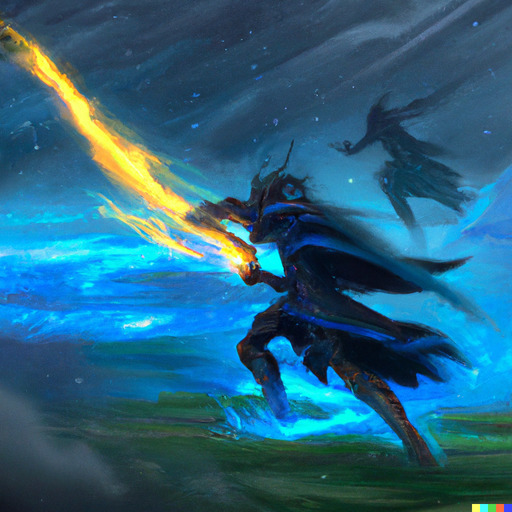
\includegraphics[width=\columnwidth]{core mechanics/spell and ritual mechanics}

    Spells and rituals are \magical abilities.
    Each spell and ritual has a name, a rank, and a specific effect.
    Spells are easy to use once they have been memorized, while rituals are complex magical ceremonies that must be followed precisely.
    In general, spells are useful in combat, while rituals tend to have more narrative effects.
    Abilities which only affect spells do not affect rituals, and vice versa.

    Every spell and ritual belongs to a specific \glossterm{mystic sphere} (see \pcref{Mystic Spheres}).
    Mystic spheres are thematically related collections of spells and rituals.

    \subsection{Learning Spells}\label{Learning Spells}
        Most characters gain access to spells through a class archetype.
        Each spellcasting class has an archetype which grants the ability to cast spells.
        The archetype will define a specific number of mystic spheres that you gain access to, and spells that you learn.
        Your rank in that archetype determines the maximum rank of spells and rituals that you can learn and use.

        When you gain access to a mystic sphere, you also automatically learn all \glossterm{cantrips} from that mystic sphere.
        Cantrips are minor spells which are easy to learn.

    \subsection{Learning Rituals}
        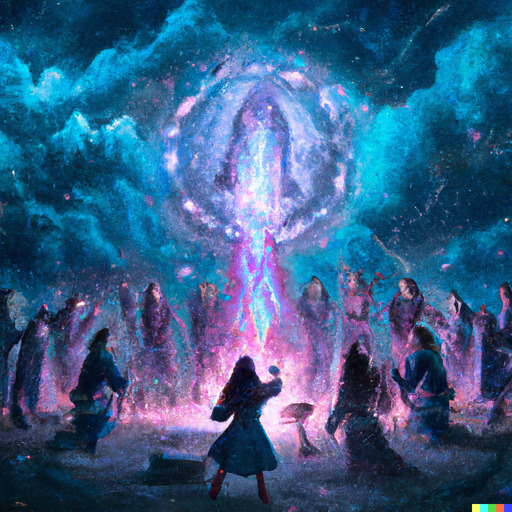
\includegraphics[width=\columnwidth]{core mechanics/rituals}

        Rituals are too complex to be memorized like spells.
        Instead, you scribe them into a ritual book which you physically carry with you.
        The spellcasting archetype of a class does not intrinsically grant access to rituals.
        Instead, most spellcasting classes can grant access to rituals through a second archetype, and only if you choose that ability.

        The number of rituals you know is not as rigidly defined as the number of spells.
        When you learn how to perform rituals, that ability will also allow you to scribe some rituals into your ritual book for free.
        However, you can also scribe new rituals into your ritual book.
        This expends precious magical ink with a value equal to a permanent item of the ritual's rank (see \tref{Item Ranks}).
        Typically, scribing a new ritual requires access to another ritual book containing that ritual.

        It is easiest to learn and perform rituals from \glossterm{mystic spheres} that you have access to.
        You can learn and perform rituals from mystic spheres that you do not have access to, but this comes with several requirements and limitations:
        \begin{itemize}
            \item Your \glossterm{magic source} must include the mystic sphere that the ritual belongs to.
            \item You treat the ritual as if it was one rank higher than its actual rank.
                This means you must have access to higher rank spells to perform it, and scribing the ritual requires more expensive magical inks appropriate to the higher rank.
            \item The ritual requires double the normal \glossterm{fatigue level} to perform.
        \end{itemize}

    \subsection{Casting Spells}
        To cast a spell, you must have that spell memorized, or you must be using a wand which grants knowledge of that spell (see \pcref{Magic Implements}).

    % The fatigue level cost for 24 hour rituals is equal to (ritual rank ^ 2) * 2.
    % Should this be specified explicitly?
    \subsection{Performing Rituals}\label{Performing Rituals}
        To perform a ritual, you must have a ritual book containing the ritual and the material components required for the ritual, if any.
        All rituals require both \glossterm{verbal components} and \glossterm{somatic components} (see \pcref{Casting Components}).
        Unlike spells, rituals can be performed as a group, with any number of ritual participants.

        \subsubsection{Ritual Participants}
            Creatures can participate in rituals even if they are unable to perform rituals themselves.
            A creature that helps perform a ritual is called a ritual participant, and the creature performing the ritual is called the ritual leader.

            Each ritual imposes some number of \glossterm{fatigue levels} on its participants.
            The ritual leader can allocate those fatigue levels among the participants.
            Normally, a ritual participant can only contribute \glossterm{fatigue levels} up to a maximum of their \glossterm{fatigue tolerance}.
            If a participant has access to the same \glossterm{magic source} as the ritual, they can contribute any number of \glossterm{fatigue levels} (until they drop unconscious).
            Creatures willing to fatigue themselves generally tire at a rate no faster than one fatigue level per ten minutes spent performing the ritual.

            The steps required to participate in rituals can be complex.
            Ritual participants must be given specific instructions for the actions they must perform during a ritual by a creature who knows how to perform the ritual.
            A creature cannot participate in rituals unless it can speak at least one language and has the fine motor control required to perform the \glossterm{somatic components} of rituals.

        \subsubsection{Changing Ritual Participation}
            Non-leading participants can freely start or stop participating in a ritual in progress.
            However, the ritual as a whole cannot be paused and restarted once in progress.
            If a ritual stops having a leader, it ends with no effect.
            The ritual leader can transfer their leadership to another creature.
            The new leader must also meet all requirements to perform the ritual themselves.
            Changing ritual participation and leadership is usually done when performing extraordinarily long or demanding rituals.

        \subsubsection{Attunement Rituals}
            Rituals with the \abilitytag{Attune} tag require a single ritual participant to \glossterm{attune} to the ritual's effect.
            Any ritual participant can attune to the effect, but only one ritual participant can attune to the effect unless otherwise noted in the ritual's description.
            For details, see \pcref{Attunement}.

        \subsubsection{Performing Rituals From Other Books}
            You can perform rituals from ritual books that you did not originally write, assuming the ritual is written in a language you understand.
            However, this is more difficult than performing rituals that you scribed yourself.
            Both the time requirement and \glossterm{fatigue level} requirement to perform a ritual in this way are doubled.

    % TODO: description
    \subsection{Categories of Magic}

        \subsubsection{Magic Sources}
            There are four \glossterm{magic sources} that characters can use to cast spells and perform rituals: arcane (cast by sorcerers and wizards), divine (cast by clerics and paladins), nature (cast by druids), and pact (cast by warlocks).
            Each magic source has a set of associated \glossterm{mystic spheres} (see Mystic Spheres, below).
            % TODO: more description

            \parhead{Characters with Multiple Magic Sources}
                Multiclass characters can have access to multiple magic sources.
                The \glossterm{mystic spheres}, spells, and rituals that character knows are tracked separately for each source of magic that character has access to.

        \subsubsection{Mystic Spheres}
            A \glossterm{mystic sphere} is a collection of thematically related magical effects that includes both \glossterm{spells} and \glossterm{rituals}.
            Each \glossterm{mystic sphere} can be associated with any number of \glossterm{magic sources}.
            The mystic spheres are listed at \pcref{Mystic Spheres}.

    \subsection{Casting Components}\label{Casting Components}
        Unless otherwise noted, all spells and rituals require \glossterm{verbal components} to cast or perform.
        In addition, spells and rituals from arcane and pact mystic sources require \glossterm{somatic components}.
        You cannot start casting a spell or performing a ritual without all required components.
        If you lose those components before the ability resolves, the spell fails with no effect.

        To provide the verbal component for a spell or ritual, you must speak in a strong voice with a volume at least as loud as ordinary conversation.
        To provide the somatic component for a spell or ritual, you must make a precise series of movements with at least one free hand.
        These movements involve your whole arm in addition to gestures with your fingers.

        \subsubsection{Somatic Component Failure}\label{Somatic Component Failure}
            Encumbrance from armor interferes with the \glossterm{somatic components} required to perform arcane spells, pact spells, and all rituals.
            When you cast a spell or perform a ritual that requires \glossterm{somatic components} while you have an \glossterm{encumbrance}, you must roll 1d10.
            If your result is less than or equal to your \glossterm{encumbrance}, the spell fails with no effect.
            When you perform a ritual, this roll must be repeated at the end of each round during the ritual.

    \subsection{Dismissal}\label{Dismissal}
        Many abilities can intentionally be ended early if you \glossterm{dismiss} it.
        When an ability is dismissed, all of its lingering effects immediately end.
        Unless otherwise noted, all \magical abilities with a duration can be dismissed, but \glossterm{mundane} abilities cannot be dismissed.
        This includes \glossterm{conditions}, \glossterm{brief} effects, and other abilities with more specific durations.
        You can dismiss abilities as a non-action that requires only mental effort.

    \subsection{Resurrecting the Dead}\label{Resurrecting the Dead}
        Several rituals have the power to restore dead characters to life.

        When a living creature dies, its soul departs its body, travels through the Astral Plane, and goes to abide on the appropriate plane or Divine Realm.
        This process is enforced by the Reapers, who escort souls to ensure they reach their intended destinations.
        Bringing a creature back from the dead means retrieving their soul and returning it to their body.

        \parhead{Deterioration of the Soul} While dead, souls gradually lose their cohesion and independent sense of self.
        A typical creature can maintain its existence in the afterlife for a number of years equal to 5 times the sum of its level and Willpower.
        This can vary significantly for individual creatures, and being tormented in the afterlife can significantly reduce this time.

        \parhead{Preventing Resurrection} Enemies can take steps to make it more difficult for a character to be returned from the dead.
        Except for \spell{true resurrection}, every ritual to raise the dead requires a body, so keeping or destroying the body is an effective deterrent.
        The \spell{soul bind} ritual prevents any sort of revivification unless the soul is first released.

        \parhead{Involuntary Resurrection} A soul cannot be returned to life if it does not wish to be.
        A soul infallibly knows the name, alignment, and patron deity (if any) of the character attempting to revive it and may refuse to return on that basis.

    \subsection{Functioning Like Other Spells}\label{Functioning Like Other Spells}
        Many spells and rituals say they ``function like'' some other spell or ritual, often with some noted changes.
        Except as otherwise noted, they retain all of the original effects and targets of the spell.
        However, they do not have the same rank upgrades as the original spell or ritual.

    \subsection{Impossible Spells and Rituals}
        When you try to use a spell or ritual in an impossible way, the ability fails with no effect.
        This most commonly happens if you attempt to declare an invalid target for a spell.

\section{Common Magical Effects}
    \subsection{Delayed and Repeated Effects}\label{Delayed and Repeated Effects}
        Some abilities cause an effect to happen in a future round, or in all subsequent rounds.
        These abilities often say that they happen ``during your action''.
        When you act during each action phase, you can decide when that effect happens, including before and after all of your other actions.
        For example, you could resolve the trigger first to see the results before deciding your actions, or you could act before the trigger to push another creature into a relevant area.

        You must still complete all of your actions, including these triggers, as part of your single turn.
        You can't resolve a trigger, then let your allies take actions, then take your own action afterwards.

    \subsection{Resurrection}\label{Resurrection}
        Some abilities can return dead creatures to life.
        This is called resurrection.

        A creature has no hit points or damage resistance when it returns to life.
        It is cured of all \glossterm{vital wounds}, \glossterm{conditions}, and other negative effects, but the body's shape is unchanged.
        Any missing or irreparably damaged limbs or organs remain missing or damaged.
        The creature may therefore die shortly after being resurrected if its body is excessively damaged.
        Some resurrection abilities can restore more damaged corpses to life, as indicated in their descriptions.

        Coming back from the dead is an ordeal.
        The creature's maximum \glossterm{fatigue tolerance} is reduced by 1.
        This penalty lasts for thirty days, or until the creature gains a level.
        If this would reduce a creature's maximum fatigue tolerance below 0, the creature cannot be resurrected.

        Resurrection is always voluntary.
        If a dead creature's soul refuses to return to life, no effect can compel it to be resurrected.
        Similarly, if a dead creature's soul has been subsumed into the planar essence of its afterlife plane, it has already been resurrected, or the soul is otherwise inaccessible, resurrection is impossible.

        Although you can resurrect creatures who have died of old age, it is usually pointless.
        They will die again before long from some malady resulting from their advanced age.

    \subsection{Shapeshifting}\label{Shapeshifting}
        When a creature shapeshifts, its physical body completely transforms into a different shape.
        It generally retains all of its original statistics and abilities, with the following exceptions.
        Some specific abilities that cause a creature to shapeshift have additional effects.
        % TODO: are more exceptions necessary?
        \begin{itemize}
            \item The creature's size changes to match the new form.
                This can change the creature's \glossterm{base speed}, Reflex defense, and other statistics as normal (see \pcref{Size Categories}).
            \item The creature's \glossterm{mundane} movement modes and natural weapons are replaced with the movement modes and natural weapons of its new shape.
            \item If the new shape is not normally capable of speech, the creature cannot speak.
                This may prevent it from casting spells with \glossterm{verbal components} and using similar abilities.
            \item The creature is limited by the number of \glossterm{free hands} present in the new form.
                In addition, it cannot gain more free hands by shapeshifting than it originally had in its base form.
                Even if you shapeshift to a form with many hands, you do not have the mental coordination necessary to use them all effectively.
            \item Any special properties that a creature had that were originally a result of its pure physical composition may be lost.
                For example, a ghost would stop being \trait{incorporeal} if it shapeshifted.
        \end{itemize}

        All of a shapeshifted creature's equipment that is physically incompatible with the creature's new shape meld into its body.
        This does not break \glossterm{attunement}, and the creature still gains the benefit of any magical properties of melded items.
        However, it does not gain the benefit of nonmagical properties from melded items.
        For example, a creature that shapeshifts into an amorphous gas would still benefit from all attuned effects from its equipped items, such as \mitem{boots of speed}.
        However, it would gain no benefit to its Armor defense or damage resistance from any melded body armor, and it would not be able to attack with any of its melded weapons.
        Items exceeding a creature's \glossterm{carrying capacity} are not melded, and simply fall to the ground in place.

        When a shapeshifted creature dies, it returns to its original form.

    \subsection{Teleportation}\label{Teleportation}
        Some abilities can \glossterm{teleport} creatures or objects.
        When you are teleported, you move through the Astral Plane and arrive at a new location.
        You can be teleported between two different locations on the same \glossterm{plane}, or between two different locations on different planes.
        If for some reason you cannot access the Astral Plane, you cannot be teleported.

        Anything being teleported must have both \glossterm{line of sight} and \glossterm{line of effect} to its destination.
        In addition, the destination of the teleportation must be an unoccupied location on a stable surface.
        That surface must be able to support the weight of the teleporting creature or object.
        If any of these conditions is not met, the teleportation fails without effect.
        Some teleportation abilities are less restricted, as indicated in their description.

        In general, you can teleport up slopes that are no more than 45 degrees.
        Steeper slopes prevent you from seeing stable ground to teleport to it.
        The GM can provide guidance for individual slopes, which may be easier or harder to navigate with teleportation.

        \subsubsection{Teleportation Noise}\label{Teleportation Noise}
            Creatures and objects that are teleported make a sound when they depart and arrive.
            This noise is caused by the displacement of air (or other substances) created by the teleportation.
            The base \glossterm{difficulty value} of an Awareness check to hear this sound for a Medium creature or object is 10.
            This difficulty value changes based on the size of the teleported creature or object:

            \begin{itemize}
                \item Fine: 30
                \item Diminutive: 25
                \item Tiny: 20
                \item Small: 15
                \item Medium: 10
                \item Large: 5
                \item Huge: 0
                \item Gargantuan: \minus5
                \item Colossal: \minus10
            \end{itemize}

        \subsubsection{Carrying Objects}
            When a creature is teleported, it can bring along equipment and held objects as long as two conditions are met.
            First, the combined weight of the objects cannot exceed the creature's maximum \glossterm{carrying capacity} (see \pcref{Weight Limits}).
            If a creature is teleported while carrying more than its maximum carrying capacity, all excess objects are left behind, starting with the heaviest object and proceeding in order of weight.

            Second, no object can extend more than two feet away from the creature's body.
            Any objects that extend beyond that distance are left behind.
            For example, a creature wearing handcuffs will arrive at its teleportation destination still wearing the handcuffs.
            However, a creature that is tied to a post by a long rope will arrive at its teleportation destination without the rope.

        \subsubsection{Astral Beacon}\label{Astral Beacon}
            Some abilities allow long-distance teleportation, such as the \ritual{overland teleportation} ritual.
            This sort of teleportation is much easier if you are travelling to an \glossterm{astral beacon}.
            The specific effects of an astral beacon are defined in the teleportation ability being used.
            An astral beacon covers an area, rather than a single point in space.

            Each astral beacon has a unique name.
            The name represents the beacon's precise location in the Astral Plane, so no two beacons can have identical names.
            For example, astral beacons created by rituals have their name defined by the precise color of ritual inks, details of drawn patterns, timing and inflection of ritual incantations, and similar subtleties.

            It is possible, though unlikely, to find astral beacons simply by wandering in the Astral Plane.
            They are similar in size and shape to \glossterm{scrying sensors}, but their appearance is visually distinct (for creatures who can see \trait{invisible} objects).
            Inspecting a beacon can reveal the location it points to, and destroying the beacon in the Astral Plane removes the astral beacon entirely.
            This is generally considered a hostile act, and may have consequences.

        \subsubsection{Horizontal Teleportation}
            Some planes have a curved primary surface.
            On those planes, ``horizontal'' teleportation isn't objectively horizontal.
            Instead, it is horizontal relative to the surface of the plane.

\section{Breaking Objects}
    There are two main ways of breaking objects.
    You can deal damage to objects with attacks, similarly to how you can deal damage to creatures.
    Alternately, you can attempt to sunder the object with sheer strength.

    \subsection{Damaging Objects}
        Objects have \glossterm{hit points} and \glossterm{damage resistance} like creatures.
        However, non-creature objects treat all damage they take as \glossterm{environmental damage} (see \pcref{Environmental Damage}).
        That means that all damage they take is reduced by their \glossterm{damage resistance} without subtracting from the remaining value of their damage resistance.

        An object becomes \glossterm{broken} if its \glossterm{hit points} are reduced to 0 (see \pcref{Broken and Destroyed Objects}).
        Objects cannot gain \glossterm{vital wounds}.
        Objects are also not normally subject to \glossterm{critical hits}.

    \subsection{Sundering Objects}
        As a standard action, you can attempt to break an object with raw strength instead of damage.
        This requires two hands.
        When you sunder an object, make a Strength check.
        The \glossterm{difficulty value} of the check is equal to the object's \glossterm{damage resistance}, \plus5 for each \glossterm{weight category} above Diminutive.

    \subsection{Broken and Destroyed Objects}\label{Broken and Destroyed Objects}
        An object that is reduced to 0 \glossterm{hit points} becomes \glossterm{broken}.
        You can destroy an object by causing it to lose additional hit points equal to ten times its maximum hit points, or by succeeding at a check to sunder the object by 10.

        \parhead{Broken Objects}\label{Broken Objects}
        Broken objects cannot be used for their intended purpose, but still retain enough of their original form to be repaired without too much work.
        For example, a broken wall lies in pieces on the ground and no longer blocks passage, but can be repaired with far less effort than would be required to create a wall from scratch.
        Magic items that are broken retain their magical properties once fixed.
        Broken (but not destroyed) objects can be repaired with the Craft skill (see \pcref{Craft}).

        \parhead{Destroyed Objects}\label{Destroyed Objects}
        Destroyed object have been damaged beyond hope of any sort of repair short of crafting the object again from raw materials.
        For example, a destroyed wall is reduced to dust or small, useless chunks of rubble.
        Magic items that are destroyed irrevocably lose their magical properties.
        The remains of a destroyed object generally occupy a space one size category smaller than the original object.
        Destroyed objects can be rebuilt with the Craft skill, but it requires significant time and investment.

    \subsection{Relative Damage Resistance}\label{Relative Damage Resistance}
        When an object would take damage from a \glossterm{strike}, if the \glossterm{damage resistance} of the attacking object or creature is lower than the damage resistance of the defender, the attacking object or creature takes the damage instead.
        For example, if you try to break a stone wall with a wooden club, the club will break instead of the wall.
        % TODO: define hardness for creatures and their natural weapons; natural weapons should generally have higher hardness than creatures to avoid hardness reflection being common

    \subsection{Breaking Equipment}\label{Breaking Equipment}
        Normally, a character's equipment cannot be damaged or otherwise affected by attacks.
        This includes worn items, anything held in your hands, and anything in a secure storage like a small backpack.
        Such items are considered \glossterm{attended}.
        They are unaffected by damage caused by area effects, and cannot be targeted individually.
        Some abilities can specifically target \glossterm{attended} objects, as indicated in their descriptions.

        \subsubsection{Loose Equipment}
            Some items are explicitly \glossterm{loose equipment}.
            Loose equipment does not gain the protections listed above while worn as equipment.
            It can be individually targeted by attackers, and is affected by area effects just like any other object in the area.

\section{Poison}\label{Poison}
    Poisons are organic substances that are dangerous to living creatures.
    They can deal damage or inflict debilitating effects.
    Some effects which are not literally poisonous, such as animal venom or fungal spores, are considered poisons.
    Poisons are not \glossterm{conditions}, and cannot be removed by abilities that remove conditions (see \pcref{Conditions}).
    Common poisons are listed in \tref{Consumables}.

    \subsection{Poison Effects}\label{Poison Effects}
        When you come in contact with a poison, you become \glossterm{poisoned}.
        As soon as you become poisoned, and at the end of each subsequent round, the poison makes an attack against your Fortitude defense.
        On a hit, the poison progresses to its next stage.
        On a critical hit, the poison progresses by two stages at once, to a maximum of the third stage.
        On a miss, you make progress towards removing the poison entirely.
        Once the poison misses you three times, you stop being poisoned.

        If you become poisoned again by the same poison, it does not intensify the effects of the poison.
        However, it cancels any progress you had made towards removing the poison.
        A poison is considered the same if it has the same name.
        If you are affected by multiple different poisons with the same name, but different accuracy bonuses, use the highest accuracy bonus.

        Poisons have no effect on non-living creatures.

        \subsubsection{Poison Stages}
            Poison effects are divided into stages.
            Becoming poisoned does not have any ill effects until the poison progresses to its first stage.

            Many poisons have a Stage 1 effect.
            This effect happens as soon as the poison's attack first succeeds against you.
            Some poisons also have a Stage 3 effect.

        \subsubsection{Poison Accuracy}
            A poison's accuracy depends on the way it was applied.
            Item-based poisons have a specific accuracy listed in their description.
            This accuracy does not depend on the skill of the creature inflicting the poison.

            Poisons inflicted by creature abilities use the creature's \glossterm{accuracy}.
            They may also have additional modifiers listed in the ability's description.
            For monsters, the poison's accuracy will be listed in the monster description.

    \subsection{Poison Transmission}\label{Poison Transmission}\label{Transmission}

        There are three ways that poisons can be contracted.

        \parhead{Contact} A contact poison affects any creature that touches it with bare skin.
        \parhead{Ingestion} An ingestion poison affects any creature that eats, drinks, or breathes it, depending on the type of poison.
        Ingestion poisons have no effect when touched or used to coat weapons.
        \parhead{Injury} An injury poison affects any creature that loses \glossterm{hit points} from something bearing the poison.
        Almost all injury poisons take liquid form, and are typically used to coat weapons.

    \subsection{Poison Forms}\label{Poison Forms}

        There are four forms of poison.

        \parhead{Gas} Gaseous poisons are difficult to store, but easy to affect foes with.
        Unless otherwise noted, a gas poison can be thrown within \shortrange, and affects a \tinyarea radius.
        \parhead{Liquid} Liquid poisons are the most common type of poison.
        Liquid poisons can be used to coat weapons, slipped into food, or simply thrown at foes.
        A dose of a liquid poison is usually about one ounce of the poison.
        Unless otherwise noted, a liquid poison has the \weapontag{Thrown} (15/30) \glossterm{weapon tag}.
        \parhead{Pellet} Some rare poisons come in small, solid pellets or cubes.
        Typically, these pellets contain a powerful liquid poison that becomes inert quickly after being exposed.
        Pellet poisons are typically applied by being slipped into food.
        \parhead{Powder} Poison in powder form cannot be used to coat weapons, but can be slipped into food or thrown at foes.
        Unless otherwise noted, a powder poison has the \weapontag{Thrown} (5/10) \glossterm{weapon tag}.

    \subsection{Coating Weapons with Poison}\label{Coating Weapons with Poison}
        As a standard action, you can coat a weapon with a single dose of a liquid contact-based or injury-based poison.
        The next time a creature takes damage from a \glossterm{strike} using that weapon, the struck creature comes in contact with the poison.
        This removes one dose of the poison from the weapon.
        Coated poisons expire and lose their effectiveness after ten minutes.

        An injury-based poison has no effect if the strike does not cause the struck creature to lose \glossterm{hit points}, but the dose is still removed from the weapon.
        For this reason, injury-based poisons are typically applied to secondary weapons that can be used after the subject is already weakened.

        A weapon can hold up to three poison doses of the same poison.
        Mixing different poison types on the same weapon is ineffective, as each poison dilutes the others.
        Only the highest rank poison on the weapon has any effect.

    \subsection{Creating Poisons}\label{Creating Poisons}

        You can use the Craft (poison) skill to create poisons with an hour of work.
        To create a poison, you must make a Craft (poison) check against a \glossterm{difficulty value} equal to 5 \add twice the poison's \glossterm{rank}.
        Success means you create the poison.
        Failure means the time is wasted and the materials are destroyed.

        Creating a poison requires special materials.
        The type of materials required, and how those materials can be acquired, depend on the type of poison:

        \begin{itemize}
            \itemhead{Alchemical} Alchemical poisons require alchemical materials.
                These normally can't be found in nature.
                In unusual circumstances, these components can be synthesized from natural chemicals or magical materials.
                This takes an hour of work, and requires a Craft (alchemy) check equal to 10 \add twice the poison's \glossterm{rank}.
            \itemhead{Plant} Plant-based poisons can typically be harvested by making a Survival check to search in appropriate terrain.
                This usually takes an hour of work.
                The \glossterm{difficulty value} of this check is usually equal to 10 \add twice the poison's \glossterm{rank}.
            \itemhead{Venom} Venom requires an appropriate body part from a creature -- often, poison it naturally produces.
                This usually takes a minute of work.
                Harvesting a body part from a creature requires a Medicine or Survival check equal to 5 \add twice the poison's rank.
        \end{itemize}
